\documentclass[a4paper]{article}
\usepackage{amsmath}
\usepackage{graphicx}

\usepackage[a4paper, margin=3cm]{geometry}

\usepackage[T1]{fontenc}
\usepackage[utf8]{inputenc}
\usepackage[serbian]{babel}
\usepackage{subfigure}	% needed for inserting figures
\usepackage{hyperref}
\usepackage{amsmath}
\usepackage{amssymb}
\usepackage[justification=centering]{caption}

\usepackage{hyperref}
\hypersetup{
    colorlinks=true,
    linkcolor=blue,
    filecolor=magenta,      
    urlcolor=cyan,
}

\begin{document}
\newcommand{\mr}[1]{\mathrm{#1}}
\renewcommand{\figurename}{Slika}
\pagenumbering{gobble}

\begin{center}
\huge{\textbf{\textsc{Integrisana kola \\za komunikacione sisteme\\Projekat za 2023/24. godinu}}}
\end{center}


\begin{center}
\large{\textbf{\textsc{Opis problema}}}
\end{center}

Projektovati širokopojasni pojačavač snage za opseg učestanosti od 3 do 6~GHz u 130~nm CMOS procesu.
Napajanje pojačavača snage može biti 1.2 ili 2.5~V u zavisnosti od izabrane topologije.
Cilj je napraviti pojačavač snage sa što većim $P_\mr{1dB}$ u zadatom frekvencijskom opsegu, uzimajući u obzir pretpostavljena ograničenja.
U okviru prve faze projekta razmatraju se širokopojasne mreže za prilagođenje, dok se u drugoj fazi projekta one koriste za projektovanje pojačavača snage.


\begin{center}
\large{\textbf{\textsc{Prva faza projekta}}}
\end{center}

U prvoj fazi projekta se razmatraju mreže za prilagođenje koje se koriste u pojačavačima snage iz druge faze projekta.
Mreže za prilagođenje se realizuju kao filtri trećeg reda koji transformišu opterećenje od 50~$\Omega$ u optimalnu impedansu $Z_\mr{opt}$. 
Pojačavači su predviđeni za rad u opsegu učestanosti od 3 do 6~GHz, i stoga se filtri projektuju za centralnu učestanost $\omega_0$ i relativni propusni opseg $\Delta$:
\begin{equation*}
\omega_0 = \sqrt{\omega_\mr{L} \omega_\mr{H}} = 2 \pi 10^9 \sqrt{3\cdot 6} = 6 \sqrt{2} \pi 10^9~\mr{rad/s}
\end{equation*}

\begin{equation*}
\Delta = \frac{\omega_\mr{H}-\omega_\mr{L}}{\omega_0} = \frac{\sqrt{2}}{2}
\end{equation*}

U prvoj fazi projekta je potrebno uraditi:

\begin{enumerate}


\item $[5]$ Na slici~\ref{fig:filter_prototype} je prikazan prototipni filtar trećeg reda. Odrediti vrednosti elemenata prototipnog filtra $g_1$, $g_2$ i $g_3$ kada je:
\begin{itemize}
\item Filtar sa Čebiševljevom karakteristikom tipa I pobuđen generatorom unutrašnje otpornosti 1~$\Omega$ u zavisnosti od parametra talasnosti $\gamma$.
\item Filtar pobuđen strujnim izvorom korišćenjem Fano metoda projektovanja u zavisnosti od parametra $x$.
\end{itemize} 
Odrediti talasnost frekvencijske karakteristike oba filtra u propusnom opsegu
\begin{equation*}
\delta = 10 \log_{10} \frac{P_\mr{max}}{P_\mr{min}}
\end{equation*}
za vrednost parametara $\gamma=1$, odnosno $x=1$.
\begin{figure}[!h]
\begin{center}
\includegraphics[scale=0.75]{fig/prototype.pdf}
\caption{Prototipni filtar.}
\label{fig:filter_prototype}
\end{center}
\end{figure}

\item $[5]$ Izračunati vrednosti elemenata denormalizovanog filtra propusnika opsega učestanosti sa slike~\ref{fig:filter_bandpass} u zavisnosti od impedanse $Z_0$, centralne učestanosti $\omega_0$, relativnog propusnog opsega $\Delta$, i vrednosti elemenata prototipnog filtra $g_1$, $g_2$ i $g_3$.

\begin{figure}[!h]
\begin{center}
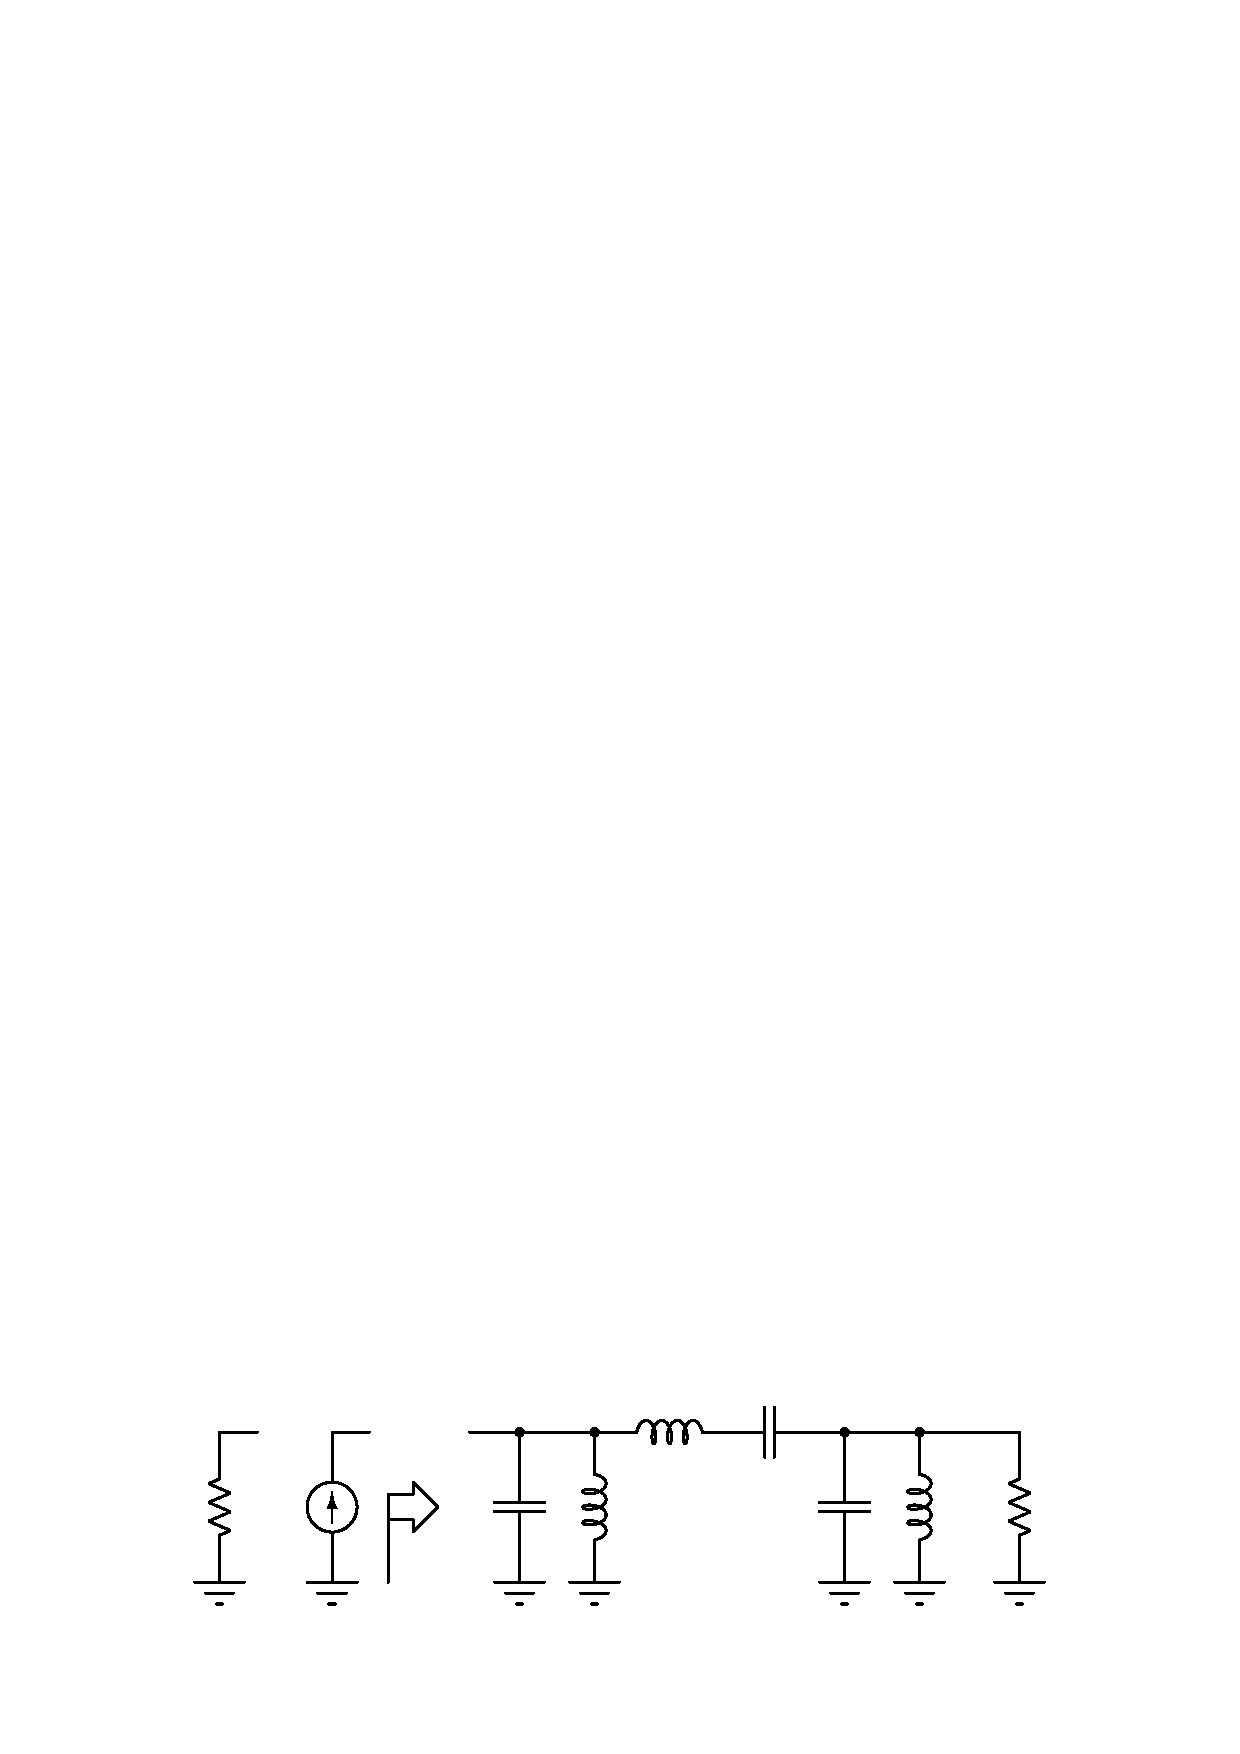
\includegraphics[scale=0.75]{fig/bandpass.pdf}
\caption{Denormalizovani filtar propusnik opsega učestanosti.}
\label{fig:filter_bandpass}
\end{center}
\end{figure}

\item $[10]$ Filtar sa slike~\ref{fig:filter_transformed} se dobija primenom kapacitivne Nortonove transformacije na kondenzatore $C_2$ i $C_3$ filtra propusnika opsega učestanosti sa slike \ref{fig:filter_bandpass}, i transformacijom $L_1$ i $L_2$ u realni transformator induktivnosti primara $L_\mr{p}$, sekundara $L_\mr{s}$, faktora sprege $k$ i rednog kalema induktivnosti $L_\mr{x}$, umetanjem idealnog transformatora $1:n_\mr{e}$, gde je
\begin{equation*}
n_\mr{e} = \frac{1}{k}\sqrt{\frac{L_\mr{s}}{L_\mr{p}}} .
\end{equation*}
Pokazati postupak transformacije i izračunati vrednosti elemenata transformisanog filtra sa slike \ref{fig:filter_transformed} u zavisnosti od $Z_0$, centralne učestanosti $\omega_0$, relativnog propusnog opsega $\Delta$, vrednosti elemenata prototipnog filtra $g_i$, faktora sprege kalemova $k$, odnosa induktivnosti sekundara i primara $L_\mr{s}/L_\mr{p}$ i faktora kapacitivne transformacije $n_\mr{c}$.

\begin{figure}[!h]
\begin{center}
\includegraphics[scale=0.75]{fig/filter_transformed.pdf}
\caption{Filtar posle primene transformacija.}
\label{fig:filter_transformed}
\end{center}
\end{figure}

\item \label{it:gamma_x_k} $[10]$ Odrediti faktor sprege $k$ realnog transformatora za koji je $L_\mr{x}=0$ u zavisnosti od elemenata prototipnog filtra $g_i$ i relativnog propusnog opsega $\Delta$. 
Izračunati minimalnu vrednost $k_\mr{min,\gamma}$ za koju je faktor talasnosti filtra sa Čebiševljevom karakteristikom $\gamma \geq 1$. 
Izračunati minimalnu vrednost $k_{\mr{min},x}$ za koju je parametar $x$ filtra sa strujnom pobudom $x \geq 1$.
Odrediti izraze $\gamma=f(k, \Delta)$ i $x=f(k, \Delta)$ pod uslovom $L_\mr{x}=0$.



\end{enumerate}

\newpage

\begin{center}
\large{\textbf{\textsc{Druga faza projekta}}}
\end{center}

Korišćenjem mreža za prilagođenje iz prve faze projekta projektovati integrisane pojačavače snage u 130 nm CMOS procesu.
Blok dijagram pojačavača snage je dat na slici \ref{fig:blockpa}.
Nije potrebno projektovati ulaznu mrežu za prilagođenje i za potrebe simulacije koristiti kolo sa slike \ref{fig:blockpa}.

\begin{figure}[!h]
\begin{center}
\includegraphics[scale=0.75]{fig/blockpa.pdf}
\caption{Blok dijagram pojačavača snage.}
\label{fig:blockpa}
\end{center}
\end{figure}

\begin{enumerate}

\item $[10]$ Odrediti optimalnu impedansu $Z_\mr{opt\times 1}$ jediničnog tranzistora za maksimalnu izlaznu snagu:
	\begin{itemize}
		\item Kaskodne konfiguracije sa napajanjem od 1.2~V, u kojoj su pojačavački i kaskodni tranzistor sa gejtom debljine $t_\mr{ox}\approx 2.6~\mr{nm}$,
		\item Kaskodne konfiguracije sa napajanjem od 2.5~V, u kojoj je pojačavački tranzistor sa gejtom debljine $t_\mr{ox}\approx 2.6~\mr{nm}$, a kaskodni tranzistor sa debljinom gejta $t_\mr{ox}\approx 7~\mr{nm}$.
	\end{itemize}
	\textit{Napomena:} U simulacijama koristiti $m=20$ puta veći tranzistor od jediničnog i preračunati optimalnu impedansu $Z_\mr{opt\times 1} = Z_{\mr{opt\times}m}/m$.
\item $[10]$ Izračunati kolika je maksimalna $P_\mr{1dB}$ snaga korišćenjem filtara iz prethodne faze projekta pod pretpostavkama $L_\mr{s}=L_\mr{p}$ i $L_\mr{x}=0$. Usvojiti da je $n_\mr{c}=n_\mr{c,max}$, i koeficijent sprege transformatora u opsegu $k=[k_\mr{min,\gamma},0.8]$, odnosno $k=[k_\mr{min,x},0.8]$. Izračunati vrednosti elemenata filtara za sve četiri kombinacije pojačavača sa napajanjem od 1.2 i 2.5 V, i obe vrste filtara.
\item $[10]$ Simulacijom odrediti $P_\mr{1dB}$ u opsegu učestanosti od 1 do 10 GHz za sve četiri kombinacije pojačavača i filtara, i nacrtati grafike.
\item (\textit{Opciono}) Projektovati ulaznu mrežu za prilagođenje koja je pogonjena idealnim naponski kontrolisanim strujnim (VCCS) generatorom. Nacrtati naponsko pojačanje za mali signal u opsegu učestanosti od 2 do 8~GHz, pod pretpostavkom da je transkonduktansa VCCS $g_m = 100~\mr{mS}$.
\end{enumerate}

\newpage

Pri projektovanju pojačavača snage potrebno je obratiti pažnju na:
\begin{itemize}
	\item Koristiti RF modele tranzistora sa širinom prsta $W_\mr{finger} \leq 5~\mu\mr{m}$,
	\item Pojačavačke tranzistore polarisati gustinom struje po širini tranzistora $100~\mu\mr{A}/\mu\mr{m} \leq I_\mr{D}/W \leq 300~\mu\mr{A}/\mu\mr{m}$,
	\item Kaskodni tranzistori sa debljinom gejta od $t_\mr{ox}\approx 2.6~\mr{nm}$ bi trebalo da budu iste širine kao pojačavački tranzistori,
	\item Kaskodni tranzistori sa debljinom gejta od $t_\mr{ox}\approx 7~\mr{nm}$ bi trebalo da budu dva do tri puta širi od pojačavačkih tranzistora,
	\item Za skaliranje širine jediničnog tranzistora koristiti faktor $m$.
\end{itemize}


\begin{center}
\large{\textbf{\textsc{Napomene}}}
\end{center}

\begin{itemize}
\item Provera ispravnosti izračunatih vrednosti elemenata se može izvršiti simulacijom $S$ parametara filtara u svim fazama projektovanja, izborom odgovarajućih vrednosti unutrašnjih otpornosti generatora.
Koeficijenti refleksije ispravno projektovanih filtara su prikazani na slici \ref{fig:filter_s11_dB}, dok je ulazna impedansa filtara na Smitovom dijagramu prikazana na slici \ref{fig:filter_s11_Smith}.

\begin{figure}[!h]
\begin{center}
\includegraphics[width=0.45\textwidth]{fig/cheby3_s11.pdf}
\hspace{5mm}
\includegraphics[width=0.45\textwidth]{fig/fano3_s11.pdf}
\caption{Koeficijenti refleksije filtara: levo - filtar sa Čebiševljevom karakteristikom, desno - filtar  pogonjen strujnim izvorom projektovan Fano metodom.}
\label{fig:filter_s11_dB}
\end{center}
\end{figure}

\begin{figure}[!h]
\begin{center}
\includegraphics[width=0.35\textwidth]{fig/cheby3.pdf}
\hspace{5mm}
\includegraphics[width=0.35\textwidth]{fig/fano3.pdf}
\caption{Ulazne impedanse filtara: levo - filtar sa Čebiševljevom karakteristikom, desno - filtar  pogonjen strujnim izvorom projektovan Fano metodom. 
Crvenom bojom je nacrtana impedansa u opsegu učestanosti od 1 do 8 GHz, dok je plavom bojom nacrtana impedansa u opsegu učestanosti od 3 do 6 GHz.}
\label{fig:filter_s11_Smith}
\end{center}
\end{figure}

	\item Izrazi za vrednosti elemenata mogu biti složeni i preporučuje se upotreba softvera za simboličku algebru, npr. SymPy, wxMaxima i sl. U direktorijumu \texttt{sympy} se nalazi Jupyter sveska sa primerom korišćenja SymPy paketa. Primer pokazuje kako se može rešiti jednačina, izvršiti smena promenljivih i rezultat pretvoriti u \LaTeX ~format.


	\item Izveštaji o prvoj i drugoj fazi projekta se pišu u formi rada za časopis u 
\href{https://journals.ieeeauthorcenter.ieee.org/create-your-ieee-journal-article/authoring-tools-and-templates/ieee-article-templates/templates-for-transactions}{MS Word ili \LaTeX~obrascu}
za IEEE Transactions on Microwave Theory and Techniques.



	\item Električne šeme se mogu nacrtati u programskom paketu 
		\href{http://opencircuitdesign.com/xcircuit/}{XCircuit}  uz pomoć 
		\href{http://tnt.etf.rs/~dgrujic/xcircuit}{biblioteke parametrizovanih simbola}.

	\item Smitovi dijagrami se mogu nacrtati izmenom \href{https://asymptote.sourceforge.io/}{Asymptote} skripti cheby3.asy i fano3.asy, koje se nalaze u direktorijumu \texttt{fig}.
			Skripte se izvršavaju komandom:
			\begin{verbatim} 
				asy -f pdf cheby3.asy 
			\end{verbatim}
	\item Grafici se mogu nacrtati pomoću Python skrite plotgraph.py,  koja se nalazi u direktorijumu \texttt{fig}. Prvi argument pri izvršavanju skripte je ime fajla sa podacima, dok su na drugom i trećem mestu \LaTeX
	~izrazi za oznake $y$ i $x$ osa, respektivno. Na primer:
		\begin{verbatim}
			python plotgraph.py cheby3_s11.csv "|S_{11}|~\mr{[dB]}" "f~\mr{[GHz]}"
		\end{verbatim}

	\item Izveštaji se predaju isključivo u PDF formatu.
\end{itemize}



%\begin{center}
%\large{\textbf{\textsc{Preporučena literatura}}}
%\end{center}
%[1] F. Harris, ''Multirate Signal Processing for Communication Systems,'' Prentice Hall, 2004.


\end{document}
